\documentclass[a4paper, 12pt]{article}

\usepackage[utf8]{inputenc}
\usepackage[portuges]{babel}
\usepackage{amsmath}
\usepackage{indentfirst}
\usepackage{graphicx}
%\usepackage[colorinlistoftodos]{todonotes}
%\usepackage{blindtext}
%\usepackage{floatrow}
\usepackage{amssymb}
%\usepackage{enumitem}
\usepackage{color}
\usepackage{aeguill}

\usepackage{underscore}
\usepackage{float}

\usepackage{xspace}
\newcommand{\gateway}{\textit{gateway}\xspace}
\newcommand{\peer}{\textit{peer}\xspace}
\newcommand{\client}{\textit{client}\xspace}
\newcommand{\cliente}{\textit{client}\xspace}

\newcommand{\peers}{\textit{peers}\xspace}
\newcommand{\clients}{\textit{clients}\xspace}
\newcommand{\clientes}{\textit{clients}\xspace}


\begin{document}
%\maketitle


\section{Introdução}

O presente relatório pretende esclarecer o funcionamento do projeto realizado no âmbito da unidade curricular Programação de Sistemas cujo objetivo consiste no desenvolvimento de um sistema de conexão entre clientes e \peers.

O projeto proposto é composto por três componentes principais: \gateway, \peer e \cliente.

Durante a execução do programa é normal que surjam múltiplos \peers e \clientes.


\section{Arquitectura e Componentes}


O sistema que se pretende desenvolver é composto, como referido, por 3 elementos principais. São eles o \peer, o \client e a \gateway. O \peer funciona como servidor do sistema recebendo e executando as intruções do \client. 
A \gateway é o primeiro contacto que ambos têm com o sistema, servindo de intermediário entre eles. 

Na figura \ref{fig:estrutura} encontra-se um esquema ilustrativo da arquitectura utilizada no projecto.


\begin{figure}[H]
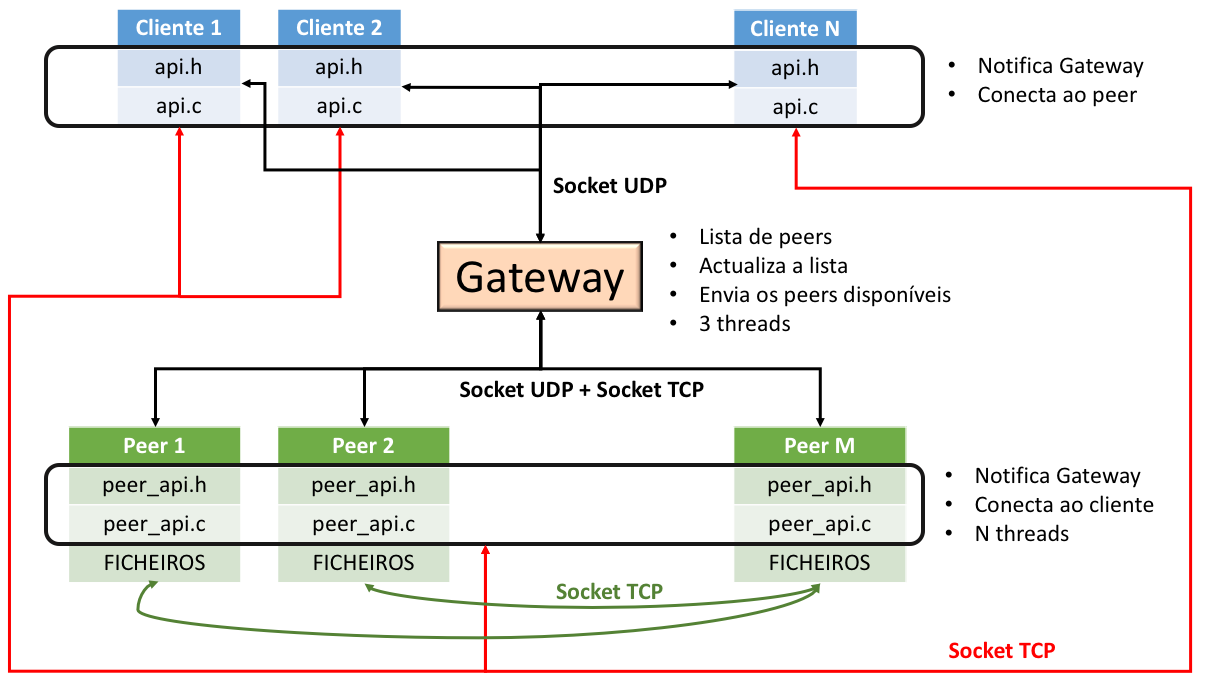
\includegraphics[width=.9\linewidth]{estrutura.png}
  \caption{Arquitectura do projecto}
  \label{fig:estrutura}
\centering
\end{figure}


\subsection{Gateway-Peer}

A comunicação entre a \gateway e um \peer pode ocorre via UDP ou TCP, em função do resultado pretendido.

Cada \peer contacta a \gateway via UDP com uma das seguintes finalidades: registar o \peer na \gateway ou obter um novo identificador para uma fotografia. 

O registo na \gateway é crucial, permitindo que um \peer seja posteriormente indicado aos \clients. No ato do registo, a \gateway atribui um identificador ao \peer, permitindo que este seja univocamente identificado. O \peer é informado do identificador que lhe foi atribuído, também via UDP, na resposta à sua tentativa de registo. A informação dos \peers registados é adicionada a uma lista na \gateway.

A \gateway funciona ainda como fornecedor de identificadores de fotografias. Optou-se por esta implementação porque todos os \peers conhecem a sua localização. Para além disso, a \gateway funciona como intermediário neste sistema, ou seja faz sentido que assuma este papel.

A \gateway utiliza também uma comunicação UDP para averiguar se determinado \peer está ou não ativo. Esta comunicação acontece quando a \gateway pretende eleger o próximo \peer que será indicado a um \client. O \peer responderá a esta mensagem, se estiver ativo, com o número de \clients que servir nesse momento. Caso não seja obtida nenhuma resposta o \peer é dado como inativo e consequentemente é removido da lista.

Um \peer pode ainda contactar a \gateway via TCP. Nesse caso, ele pretende obter a lista dos restantes \peers registados. Assim sendo no inicio da ligação o \peer que a invocou apresenta-se com o identificador que lhe foi atribuído aquando do seu registo. Logo de seguida a \gateway enviará a lista dos restantes \peers que se encontram registados e terminará a ligação. Optou-se por uma ligação TCP para esta situação especifica uma vez que a quantidade de informação a transmitir pode ser, potencialmente, elevada. Assim sendo, uma conexão fidedigna que garanta a entrega das mensagens é mais adequada e menos propícia a erros.


\subsection{Gateway-Cliente}

Um \client apenas contacta a \gateway para obter o endereço de um \peer disponível. Esta comunicação é realizada via UDP.

A \gateway elege o \peer que, nesse momento, sirva o menor número de \clientes proporcionando assim uma distribuição uniforme dos \clientes pelos \peers.

\subsection{Peer-Cliente}



Assim que um \cliente e \peer se conectam, via TCP, o \cliente poderá fazer-lhe os pedidos, relativos à galeria, diretamente.

Todos pedidos estão identificados e as mensagens enviadas de um \cliente para um \peer devem iniciar-se por esse identificador. De seguida, o cliente envia informação relativa a esse pedido e o $peer$ executa-o.

\subsection{Peer-Peer}

Existem duas situações em que um \peer se comporta como \cliente.

A primeira ocorre antes de determinado \peer se registar na \gateway. Antes desse registo, o \peer contacta um \peer já registado (contactando a \gateway) de forma a obter o estado atual do sistema.


A segunda ocorre sempre que determinado \peer recebe uma instrução de um \client que provoque alterações ao sistema. Nesse caso, o \peer contacta a \gateway para obter a lista dos restantes \peers registados, conecta-se a eles como cliente, e replica a informação que recebeu. Essa ligação é terminada logo de seguida.




\section{Threads}
\subsection{Gateway}

Na gateway verifica-se a existência de 3 threads.

A thread principal do processo abre as sockets necessárias, inicializa a lista de \peers, lança duas outras threads, responsáveis pelo tratamento da informação recebida por UDP. A thread principal é ainda responsável pelo tratamento dos pedidos TCP.

São criadas duas threads para lidar com mensagens UDP. Uma delas é dedicada aos \clientes e a outra dedicada aos \peers. Estes threads são inicializados pela função 
\texttt{pthread_create} que recebe como argumento a socket respetiva, inicializada pelo thread principal. Ambos os threads, aguardarão indefinidamente por uma mensagem UDP e trata-la-ão adequadamente.

O thread principal aguarda indefinidamente por uma conexão TCP de um \peer. No entanto , este thread define antes de tudo, um handler para sinais to tipo \texttt{SIGINT}. Assim que este sinal ocorrer, força o término dos threads que lançou com recurso à função \texttt{pthread_cancel}, aguarda que ambos seja terminados corretamente recorrendo a \texttt{pthread_join} e por último fecha as sockets e liberta memória alocada para a lista.


\subsection{Peer}

A thread principal começa por abrir as sockets TCP e UDP e inicializar o vetor de fotografias conectando-se como cliente a um \peer já existente. Obtém ainda o seu identificador ao registar o \peer na \gateway. Analogamente à \gateway, o thread principal também define um handler para sinais do tipo \texttt{SIGINT}.

De seguida, o thread principal inicializa um novo thread, com \texttt{pthread_create}, responsável por receber as mensagens UDP vindas da \gateway. Este thread receberá apenas mensagens para confirmar se o \peer se encontra ativo.

O thread principal ficará responsável por receber ligações TCP provenientes de clientes. Por cada nova ligação recebida, este thread abre um novo que fica responsável por manter essa ligação. Deste modo, o thread principal está sempre disponível para atender novos pedidos de ligação. O thread principal mantém ainda uma lista com o threads ativos. Caso a ligação TCP seja terminada normalmente, o próprio thread remove-se desta lista e liberta a sua memória recorrendo à função \texttt{pthread_detach}. Caso o sinal \texttt{SIGINT} seja acionado, o thread principal termina todos os threads da lista, fecha as sockets e liberta a memória alocada à semelhança do que acontece na \gateway.


\section{Morte de peers}
\par A $Gateway$ é informada da morte de um $peer$ apenas quando o tenta contactar, aquando de um pedido de cliente, e é aí que efectua a remoção do $peer$ da lista.



\section{Estruturas}

Existe apenas uma estrutura que é partilhada entres os vários threads tanto no \peer como na \gateway. Essa estrutura é a lista.

Embora os elementos armazenados pela lista sejam diferentes é a própria lista que potencialmente sofre problemas de sincronização. Na \gateway é partilhado entre threads a lista que armazena informação sobre os \peers. Uma vez que só é possível adicionar ou remover um \peer da lista, apenas há problemas de sincronização no acesso à lista. O mesmo acontece para a lista de threads no \peer. Quanto à informação sobre uma foto, o único parâmetro que pode ser editado depois de adicionada a lista é lista de keywords, que é ela própria uma lista.

Ou seja, os problemas de sincronização resumem-se à lista utilizada.

\subsection{Sincronização}

Relativamente à sincronização é necessário garantir que cada thread não avançara para o nó seguinte da lista se este estiver a ser escrito ou apagado. Não havendo nenhum problema quanto à leitura.

De modo a aplicar esta restrição são utilizados \textit{read/write locks} em pontos chave da lista. Cada nó da lista terá um lock relativo à posição seguinte, sendo que o lock relativo à primeira posição se encontra na estrutura inicial da lista. Sempre que se pretende obter a posição seguinte é necessário envolver essa acesso entre as funções \texttt{pthread_rwlock_rdlock} e \texttt{pthread_rwlock_unlock}, garantindo que nenhum outro processo está a escrever nesse nó simultaneamente. Analogamente, sempre que se pretenda editar o nó seguinte, numa remoção ou adição da lista, é necessário envolver essa edição entre as seguintes funções: \texttt{pthread_rwlock_wrlock} e \texttt{pthread_rwlock_unlock}. Garantindo assim que nenhum outro thread está a ler ou a escrever nesse nó simultaneamente.

\section{Replicação}

Como já explicado, quando o \peer recebe um instrução vinda de um cliente que provoca alterações ao sistema, este contacta a \gateway para obter a lista de \peers registados. De seguida conecta-se a cada um deles como \cliente e reenvia a informação que acabou de receber. A ligação criada é imediatamente terminada.


\section{Download de informação}
\par Por forma a ocorrer o download da informação presente nos $peers$ para um novo $peer$ este primeiramente comporta-se como um cliente, pedindo à $Gateway$ um $peer$ disponível.
\par Se existir, o $peer$ novo é ligado ao $peer$ fornecido pela $Gateway$, que serializa a lista e envia para o primeiro para que possa replicá-la.
\par Por fim é feito o registo do $peer$.


\newpage
\section{Critérios}
 Relativamente aos critérios de avaliação, na versão submetida pelo $fenix$, foram cumpridos os seguintes requisitos:
 \begin{itemize}
 \item (1) Implementação da API do cliente a contactar com um $peer$
 \item (2) Múltiplos $peers$ e contacto com a $gateway$
 \item (3) Múltiplos $peers$, contacto com a $gateway$ e $download$ da informação
 \item (4) Verificação da morte dos $peers$
 \item (5) Geração do identificador da imagem
 \item (8) Tranferência de imagens
 \end{itemize}




\end{document}
